\chapter{Application Design}\label{chapter::decentralizedapps}

\section{Introduction}
	An Application software or \textit{app} is a computer program designed to perform a specific set of tasks or actions for the end user. There are countless number of applications in use today and the majority of them are web applications following a centralized client-server model\cite{raval2016decentralized}.
	
	\begin{figure}[h]
		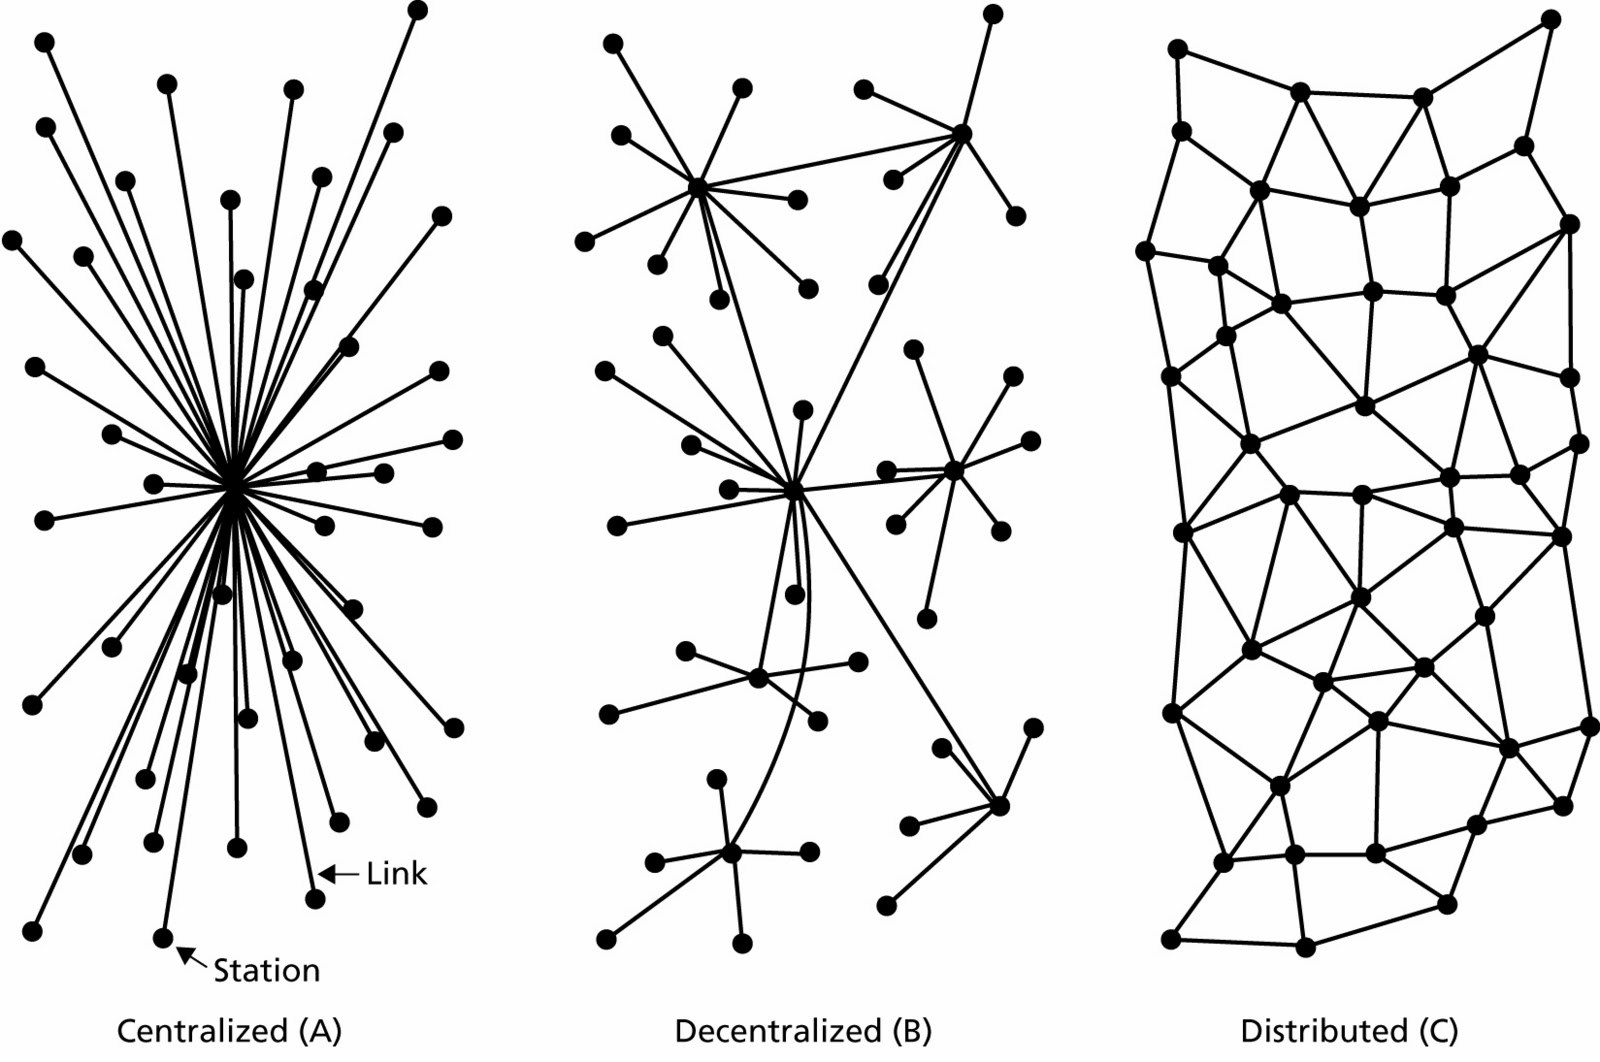
\includegraphics[width=\linewidth]{figures/network-models}
		\caption{\label{fig:applications} The three way of modeling web applications}
	\end{figure}
	
	Figure~\ref{fig:applications} shows a visual representation of three different ways of modeling web applications\cite{baran1964distributed}. Here, \textit{Centralized} and \textit{Decentralized} refers to level of control, while \textit{Distributed} refers to differences of location. Both centralized and decentralized systems can be distributed as well.
	
	\subsection{Centralized}
	It's currently the widespread way of building software applications. In this model a central server control the flow of information and governs the operation of individual units. Since the control is centralized, these types of systems suffer from single point of failure risk.
	
	\subsection{Distributed}
	In a Distributed model, the control still resides with a central server, however, the computation is spread across multiple nodes or servers.
	
	\subsection{Decentralized}
	In a Decentralized model, there is no central point of control as it's spread across all the servers running the application. Applications built using this model don't have a single point of failure and are inherently fault tolerant.

\section{Enabling Technologies}
	The document \textit{Information Management: A Proposal\cite{berners1989information}} written by \textit{Sir Tim Berners-Lee\footnote{\url{https://www.w3.org/People/Berners-Lee/}}} conceived the ideas for what would become the WorldWideWeb. It's main goal was to enable information exchange between computers in an accessible way at CERN\footnote{\url{https://home.cern/}}.
	
	HTML\footnote{\url{https://developer.mozilla.org/en-US/docs/Web/HTML}}, URI\footnote{\url{https://tools.ietf.org/html/rfc3986}} and HTTP\footnote{\url{https://tools.ietf.org/html/rfc2616}} were the fundamental technologies that defined the foundation of the Web. HTTP connected every computer on the planet with a common protocol. The HTTP protocol guidelines defined a set of trusted servers that translated a web address into a server address. Furthermore, HTTPS\footnote{\url{https://tools.ietf.org/html/rfc2818}} added another layer of trusted servers and certificate authorities. People would host personal servers for others to connect to, and everyone owned their data\cite{raval2016decentralized}. As the Web evolved, applications servers\footnote{\url{https://en.wikipedia.org/wiki/Application_server}} became the common way of interactive with the Web and the centralized model of data ownership as we know it today was born\cite{raval2016decentralized}. It was conceptually and programmatically easier to maintain an application server and profit from user's data that utilize it.
	
	Blockchain is the primary technology that enables the creation of applications with a decentralized model of data ownership. It puts the users of an application in control of their data thereby enabling a more open Web, as it was originally intended\footnote{\url{https://webfoundation.org/about/vision/history-of-the-web/}}.
	
	The blockchain helped solve the Byzantine Generals Problem\cite{lamport1982byzantine}. This problem describes a situation where all participating nodes in a distributed network must agree upon every message that is being transmitted between nodes, but where some of the nodes are corrupt and disseminating false information or are unreliable. This agreement is called as \textbf{consensus}. With Bitcoin\cite{nakamoto2008bitcoin}, decentralized consensus became possible. Agreement is achieved in the Bitcoin network by way of \textit{proof-of-work\footnote{\url{https://en.bitcoin.it/wiki/Proof_of_work}}} consensus mechanism which is resistant to Sybil Attack\cite{douceur2002sybil}. Proof-of work is both computationally and energy expensive; other consensus mechanism such as \textit{proof-of-stake\footnote{\url{https://en.bitcoin.it/wiki/Proof_of_Stake}}} relies on stake in the system instead of computational power.
	
\section{Concepts}
	There are five concepts in a web application that have traditionally been implemented in way that puts control with a centralized entity: data, identity, value, computing and bandwidth\cite{raval2016decentralized}. Each of these require trust in a 3rd party - a trust which can be betrayed. Recent advancements in distributed-system technology can put users in control of these things. Below sections describes each concept in detail and shows how one can build applications in a way such that centralized control is not required.

	\subsection{Data}
		Data is the most important concept in any web application. First, let's look at how traditional web applications interact with data. Whenever, a user logs into an application, the application connects to a remote server and sends the authentication details. These details lets the server know which user is interacting with the application. Once authenticated, the user data is fetched from the remote storage and displayed to the user. All complex computations and data storage occurs on dedicated servers maintained in the cloud.
		
		\begin{figure}[h]
			\centering
			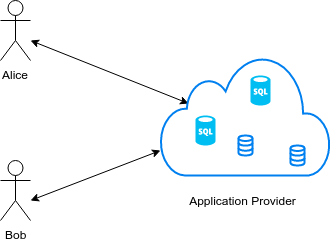
\includegraphics[width=200pt, height=150pt]{figures/traditional-app}
			\caption{\label{fig:traditional-app} How traditional web applications work}
		\end{figure}
		
		Figure~\ref{fig:traditional-app} shows how users interact with a traditional web application. Whenever, Alice wants to interact with Bob, she sends a message to the application server which then delivers the message to Bob. There is no direct path between Alice and Bob. This results in centralization where the provider acts as an intermediary between Alice and Bob's interaction; effectively governing how data is stored and shared among them.
		
		This model of application interaction requires that we trust the providers with out data and hope that they won't misuse or sell our data without our permission. Since revelations by Edward Snowden\cite{greenwald2014no}, we now know that trust can, has and will be broken as long as we entrust our data to a central entity\cite{raval2016decentralized}. Centralized stores of data also serve as a tool for surveillance, allowing big entities to monitor our internet behaviour without our knowledge. Cloud providers, despite having a distributed backend, are centrally owned.
		
		Additionally, as we move from a labor-based economy to an information-based economy, data will become the primary form of value. Therefore, its important that we not only possess our data, but own it as the world evolves. An ideal solution that enables this should provide a way of storing data in a decentralized way that is robust and as trustless as possible\cite{raval2016decentralized}.
	
		\subsubsection{1: Storing Data Directly in a Blockchain}
		This method does solves the decentralization of data as everyone who has copy of the Blockchain is storing the data but cannot alter it. The data can be encrypted such that it can only be accessed by someone having the private key. However, Blockchains were not meant for storing large amounts of data. It was designed for storing simple transactional logs, as its evident from looking at the Bitcoin Blockchain where individual records are in bytes\footnote{\url{https://en.bitcoin.it/wiki/Transaction}} and therefore cannot hold much data. Moreover, the Blockchain architecture implies that each node in the network must store a complete copy of the Blockchain. Therefore, storing a significant amount of data on a Blockchain is both expensive and impractical.
		
		\subsubsection{2: Storing Data in a Distributed Hash Table}
		DHTs ensure data resiliency by enabling easy distribution and indexing of data. Early peer-to-peer (P2P) filesharing applications like KaZaA\cite{good2003usability}, Napster\cite{ku2002creative} and Gnutella\cite{ripeanu2002mapping} used their own versions of DHTs with a varying degree of decentralization. Some had centralized trackers to monitor the movement of data, while some had central sources from which all data must pass, leaving them with single point of failure\cite{raval2016decentralized}.
		
		BitTorrent\cite{cohen2008bittorrent} was the first protocol to popularize DHT for sharing of large files. As of 2013, BitTorrent has 15–27 million concurrent users at any given time\cite{wang2013measuring}. The BitTorrent Mainline DHT serves as a decentralized data store with centralized trackers to monitor the network. It uses a tit-for-tat strategy between seeders and leechers to maximize the bandwidth of data distribution. This makes the BitTorrent protocol the de facto method for transfer of large datasets over the web. However, using BitTorrent as a data store is not feasible as there is no incentives for nodes to store a data leading to \textit{data impermanence}.
		
		\subsubsection{3: Storing Data in a Cloud in Encrypted Containers}
	
	\subsection{Identity}
	
	\subsection{Value}
	
	\subsection{Computing}
	
	\subsection{Bandwidth}